%=======================================================
\section{VMware}
%=======================================================
Virtualisierung ist ein wichtiger Bestandteil heutiger IT-Landschaften geworden. In Version 1.12 wurde aus diesem Grund das \emph{Provisioning} erweitert. Es ist nun möglich direkt virtuelle Maschinen (VM) und Host-Systeme aus einer \emph{VMware} basierenden Virtualisierung in \emph{OpenNMS} zu importieren.

Typischerweise sind diese Informationen über das \emph{vCenter} zugänglich. Leistungsdaten können dort allerdings nur über einen sehr begrenzten Zeitraum gespeichert werden.

%=======================================================
\subsection{Vorbereiten VMware vCenter}
%=======================================================

\begin{figure}[H]
	\centering
	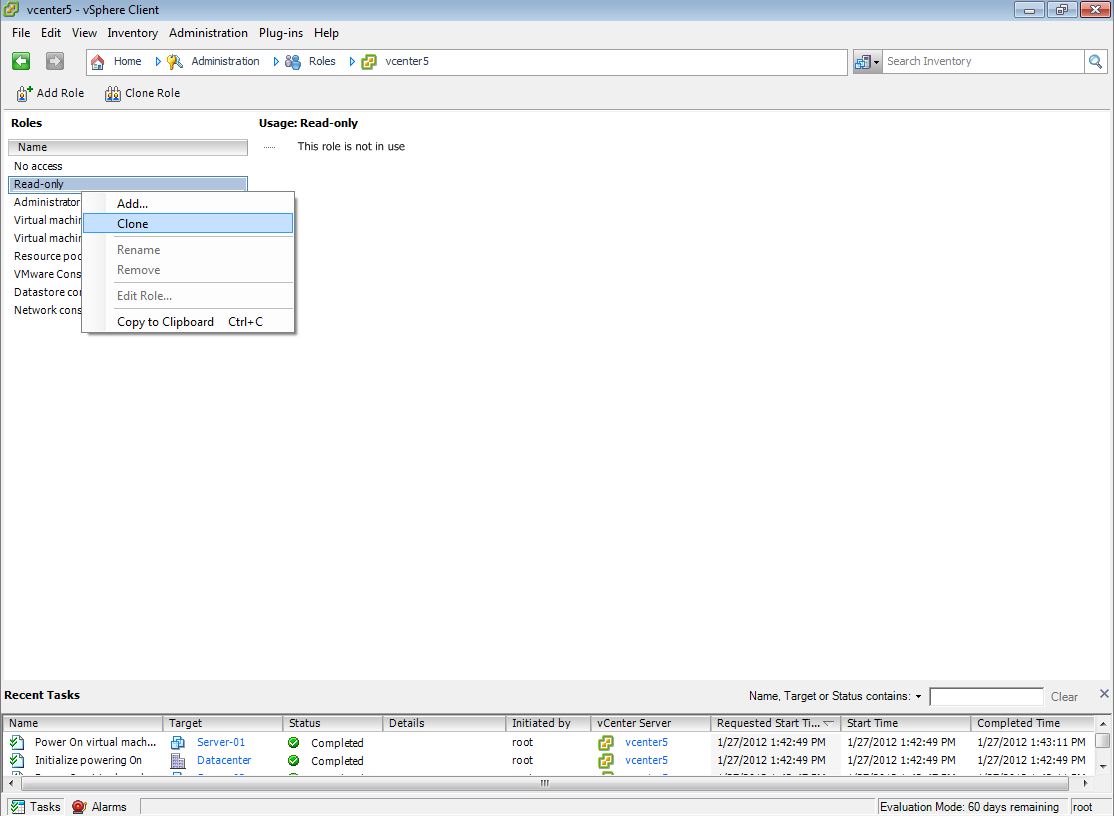
\includegraphics[width=1.0\textwidth]{images/3rd-party/vmware/0-cloning}
	\caption{Duplizieren einer \emph{Read-Only} Rolle in \emph{vCenter}}
	\label{pic:vmware-cloning}
\end{figure}

\begin{figure}[H]
	\centering
	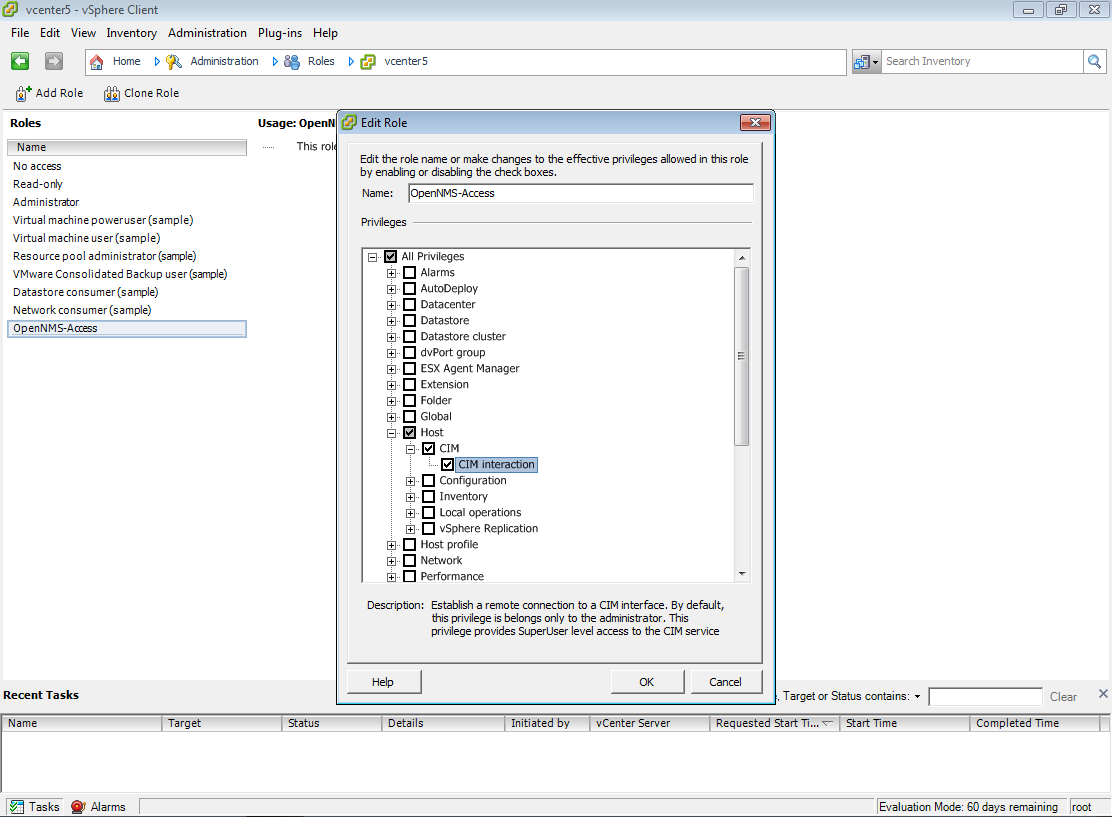
\includegraphics[width=1.0\textwidth]{images/3rd-party/vmware/1-editing}
	\caption{Duplizieren einer \emph{Read-Only} Rolle in \emph{vCenter}}
	\label{pic:vmware-editing}
\end{figure}

\begin{figure}[H]
	\centering
	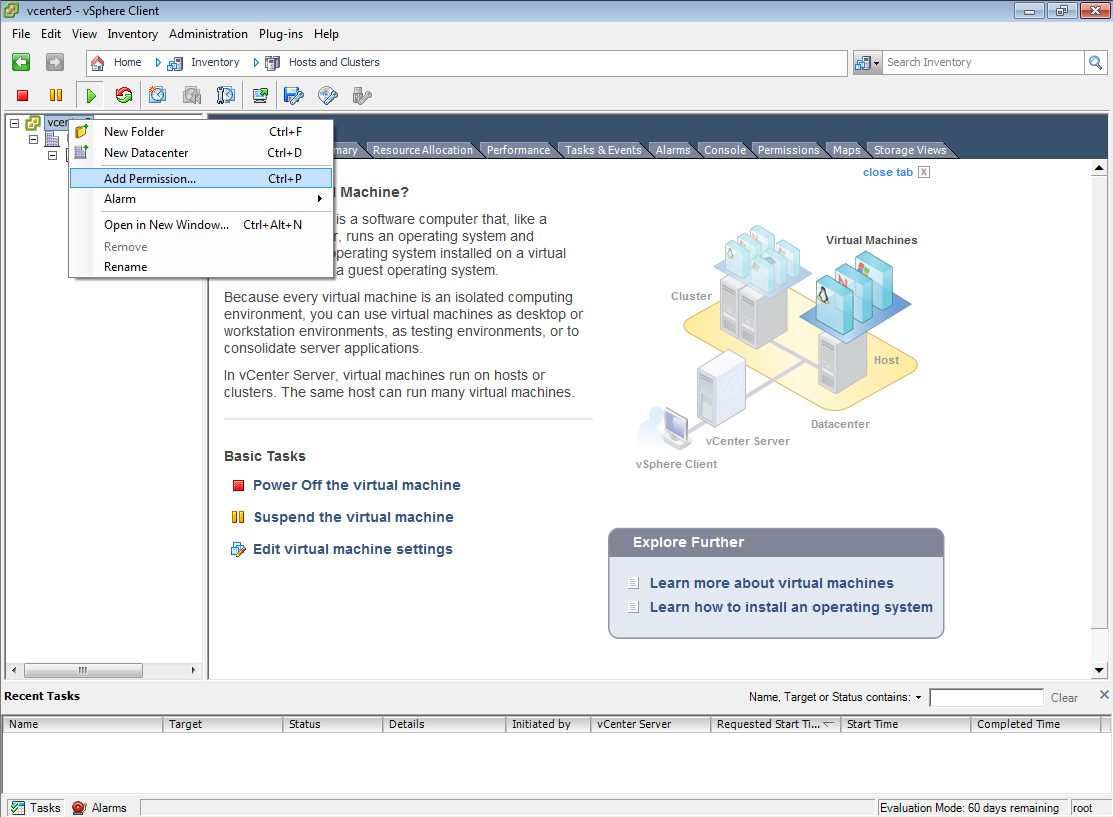
\includegraphics[width=1.0\textwidth]{images/3rd-party/vmware/2-permission}
	\caption{Duplizieren einer \emph{Read-Only} Rolle in \emph{vCenter}}
	\label{pic:vmware-permission}
\end{figure}

\begin{figure}[H]
	\centering
	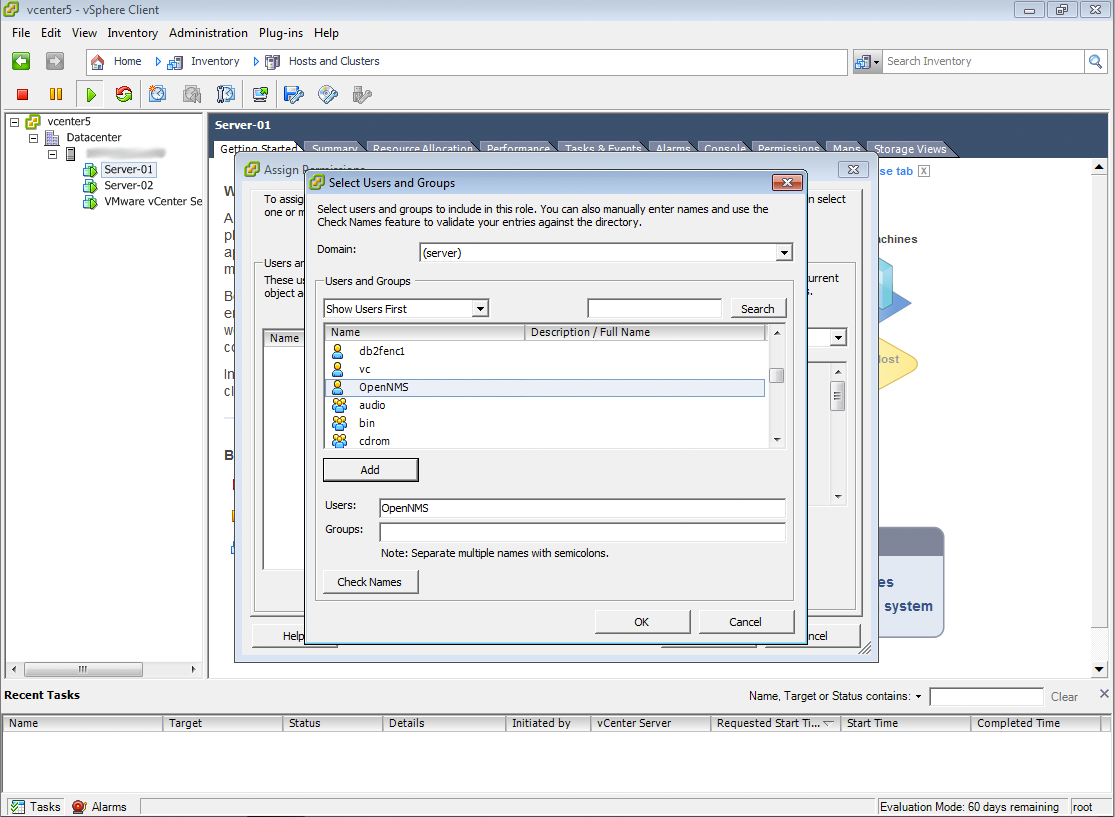
\includegraphics[width=1.0\textwidth]{images/3rd-party/vmware/3-adding}
	\caption{Duplizieren einer \emph{Read-Only} Rolle in \emph{vCenter}}
	\label{pic:vmware-adding}
\end{figure}

\begin{figure}[H]
	\centering
	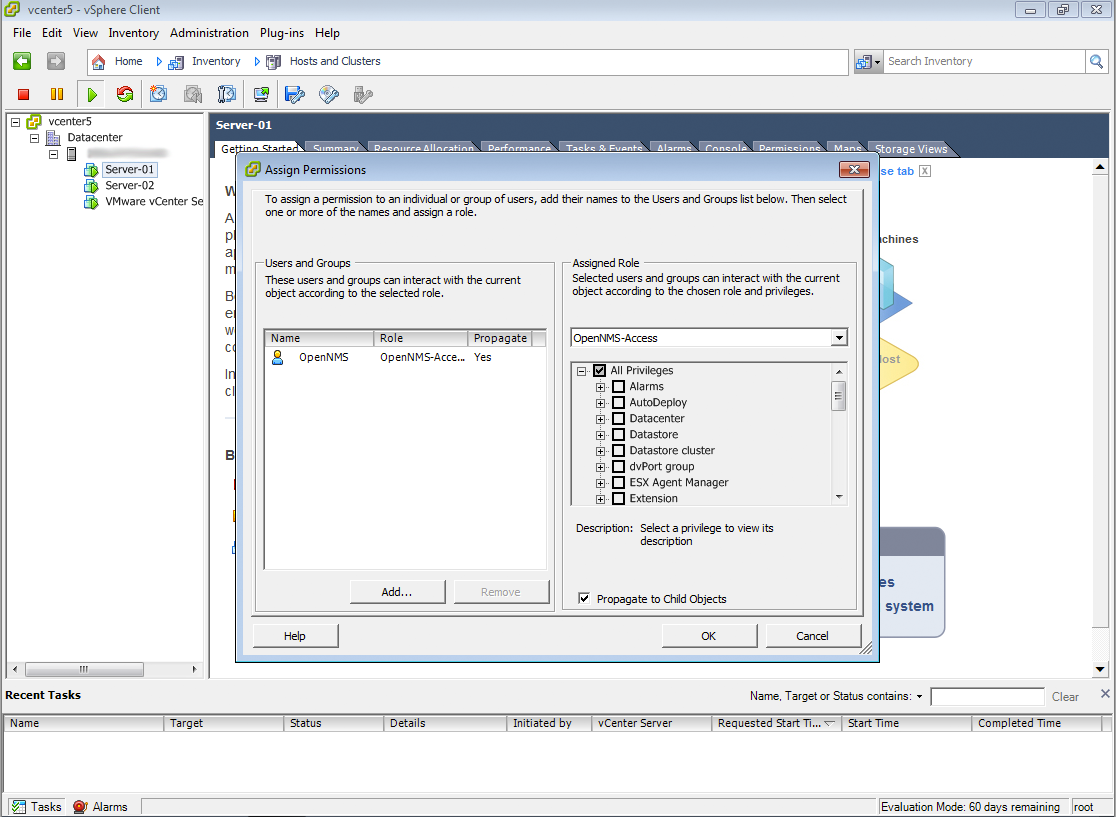
\includegraphics[width=1.0\textwidth]{images/3rd-party/vmware/4-ok}
	\caption{Duplizieren einer \emph{Read-Only} Rolle in \emph{vCenter}}
	\label{pic:vmware-ok}
\end{figure}

\begin{figure}[H]
	\centering
	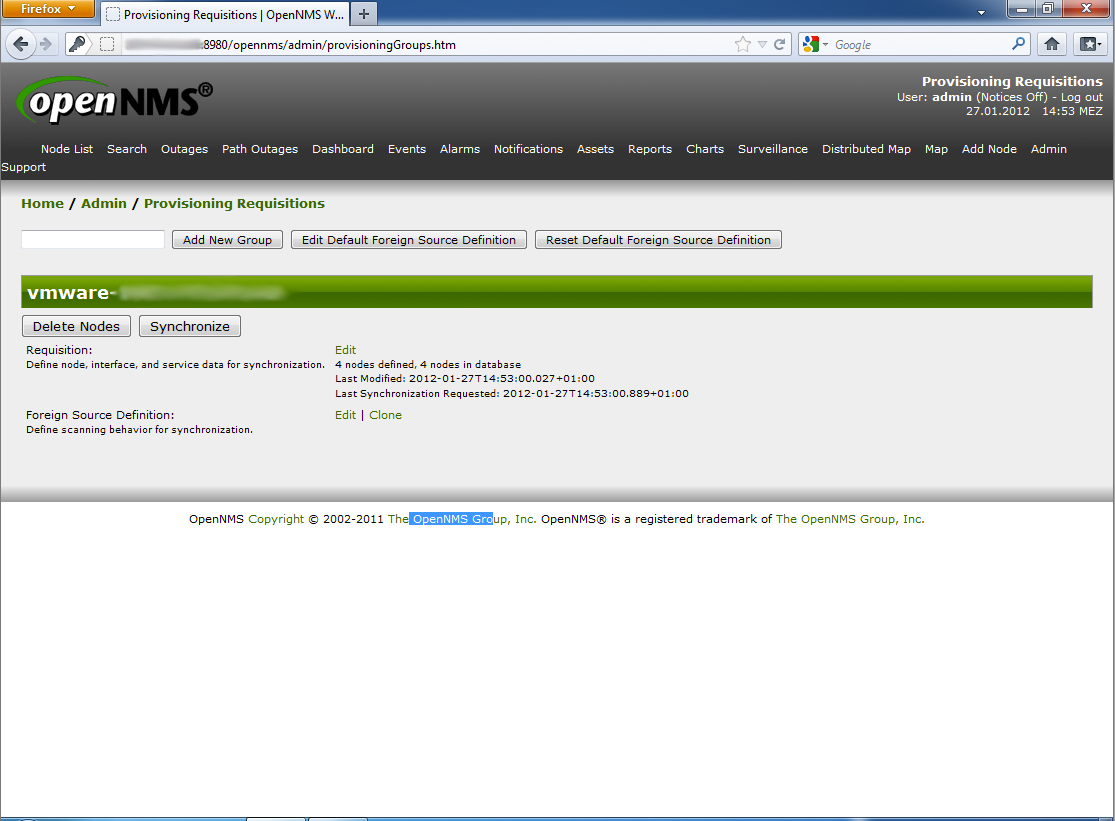
\includegraphics[width=1.0\textwidth]{images/3rd-party/vmware/5-provisioning}
	\caption{Duplizieren einer \emph{Read-Only} Rolle in \emph{vCenter}}
	\label{pic:vmware-provisioning}
\end{figure}

\begin{figure}[H]
	\centering
	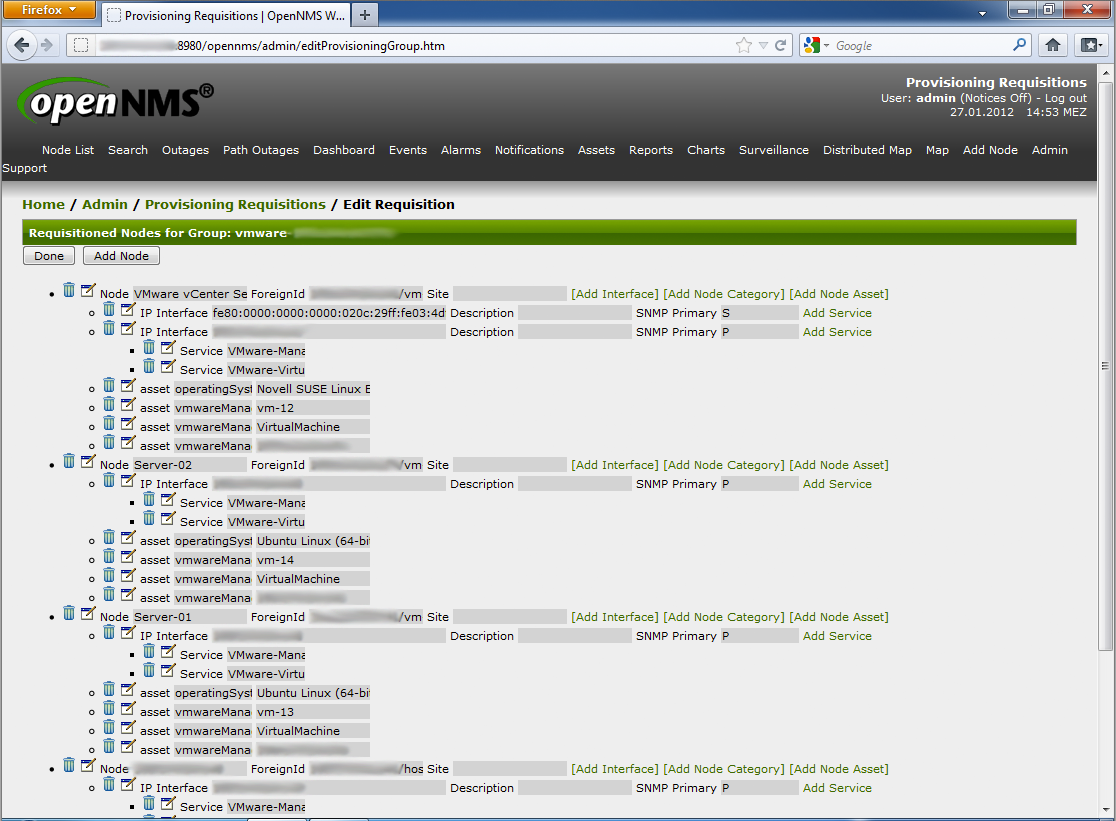
\includegraphics[width=1.0\textwidth]{images/3rd-party/vmware/6-group}
	\caption{Duplizieren einer \emph{Read-Only} Rolle in \emph{vCenter}}
	\label{pic:vmware-group}
\end{figure}

\begin{figure}[H]
	\centering
	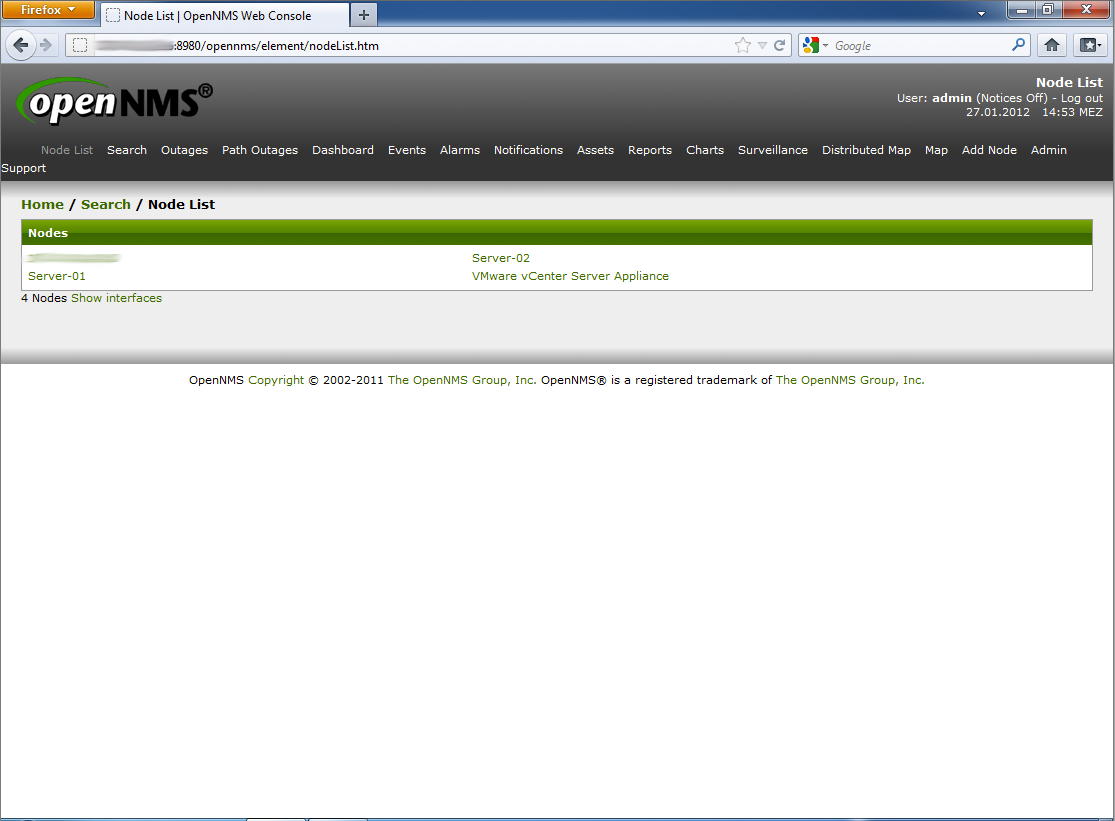
\includegraphics[width=1.0\textwidth]{images/3rd-party/vmware/7-nodes}
	\caption{Duplizieren einer \emph{Read-Only} Rolle in \emph{vCenter}}
	\label{pic:vmware-nodes}
\end{figure}

\begin{figure}[H]
	\centering
	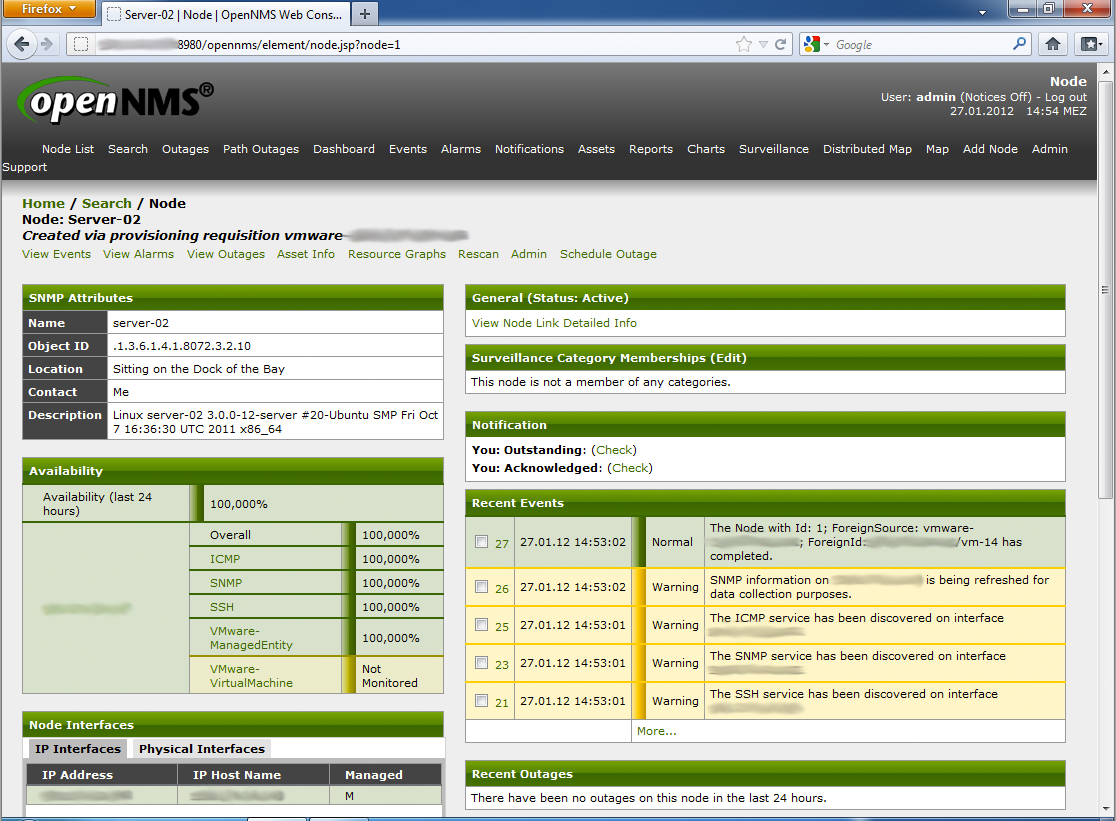
\includegraphics[width=1.0\textwidth]{images/3rd-party/vmware/8-detail}
	\caption{Duplizieren einer \emph{Read-Only} Rolle in \emph{vCenter}}
	\label{pic:vmware-detail}
\end{figure}


%=======================================================
\subsection{VMware Provisioning Adapter}
%=======================================================
In \emph{VMware vCenter} werden alle Komponenten verwaltet, die in der virtuellen Umgebung eingesetzt werden. Dort werden neben den VMs und Host-Systemen auch Leistungsdaten und der Hardwarestatus der Host-Systeme ermittelt und zur Verfügung gestellt. Um die VMs und Host-Systeme von einem bestehenden \emph{vCenter} zu importieren wurde das \emph{Provisioning} um einen \emph{Requisition-Handler} erweitert. Dieser verbindet sich zum \emph{vCenter} und liest dort alle notwendigen Informationen der VMs und Host-Systeme und überführt diese in das \emph{OpenNMS Model} für den Import.

Für den Import werden die folgenden Informationen aus vCenter ausgelesen:
\begin{itemize}
  \item \textit{}
\end{itemize}

\begin{figure}[H]
	\centering
	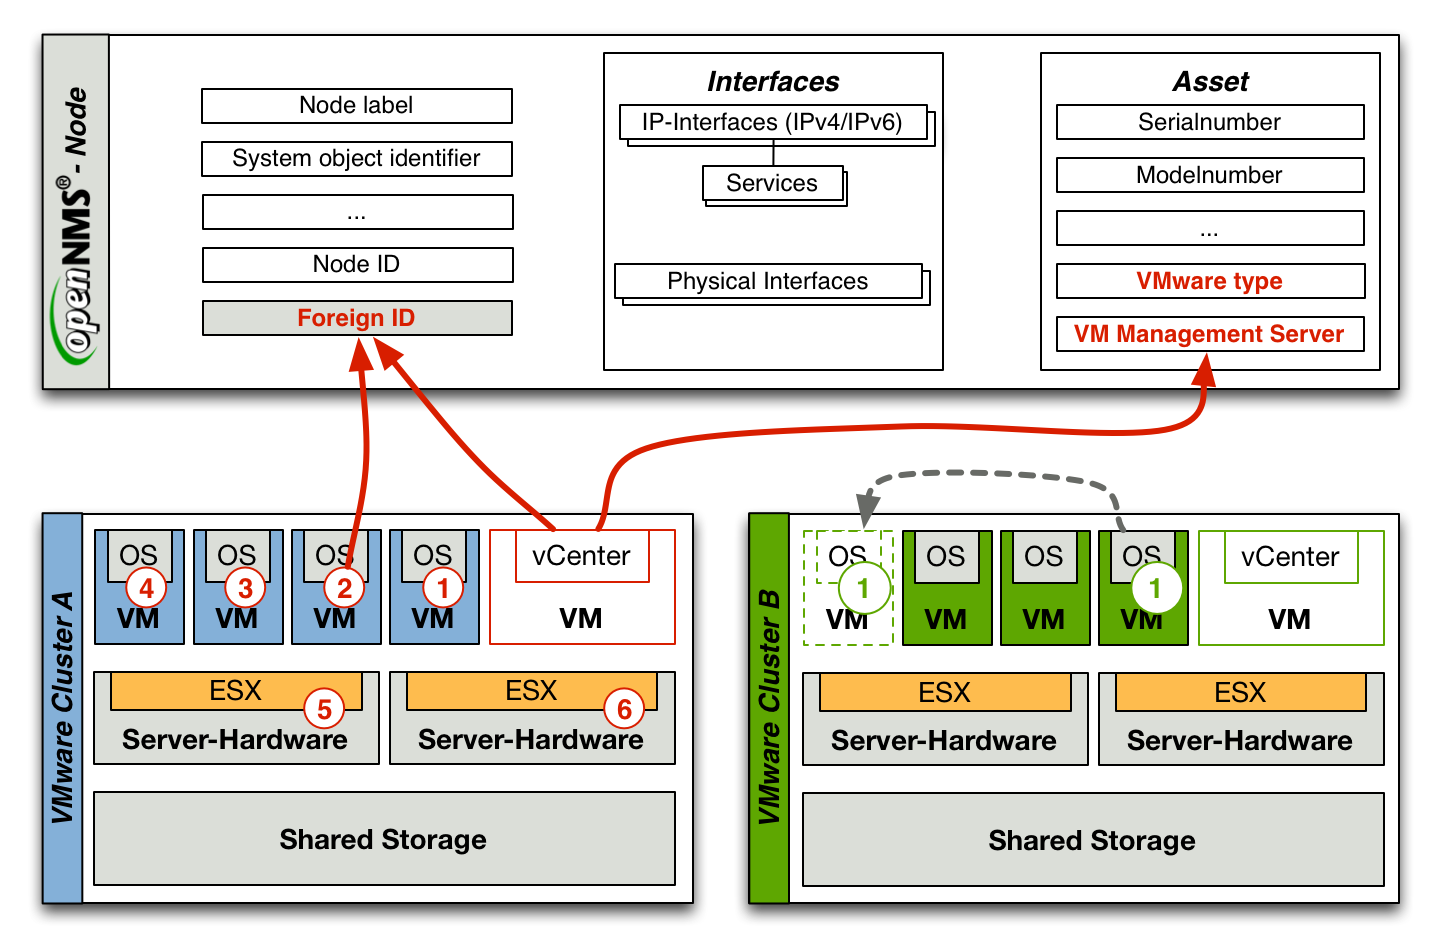
\includegraphics[width=1.0\textwidth]{images/3rd-party/vmware/vmware-cluster}
	\caption{\emph{Provisioning} mit mehreren \emph{VMware Clustern}}
	\label{pic:lab}
\end{figure}


%=======================================================
\subsection{Leistungsdaten von VMware Umgebung}
%=======================================================

%=======================================================
\subsection{Hardwarestatus von VMware Hosts}
%=======================================================

%=======================================================
\subsection{VMware und die Topology Karte}
%=======================================================